% !TeX program = xelatex 
\documentclass{hitreport}
\usepackage{url}
\usepackage{algorithm}  
\usepackage{algpseudocode}  
\usepackage{amsmath}
\usepackage{cite}
\usepackage{threeparttable}
\usepackage{subfig}
\renewcommand{\algorithmicrequire}{\textbf{Input:}}  % Use Input in the format of Algorithm  
\renewcommand{\algorithmicensure}{\textbf{Output:}} % Use Output in the format of Algorithm  

% =============================================
% Part 0 Edit the info
% =============================================

\major{计算机科学与技术}
\name{孙骁}
\title{机器学习实验报告}
\stuid{1180300811} % 学号
\college{计算学部}
\date{2020年10月6日}
\lab{} %实验地点
\course{机器学习}
\instructor{刘扬}
% \grades{}
\expname{多项式拟合正弦曲线} %实验名称
% \exptype{} % 实验类型
% \partner{} % 同组学生名字

\begin{document}
% =============================================
% Part 1 Header
% =============================================

\makecover

% =============================================
% Part 2 Main document
% =============================================

\section{实验目的和要求}

\subsection{实验目的}
掌握最小二乘法求解(无惩罚项的损失函数)、掌握加惩罚项(2范数)的损失函数优化、梯度下降法、共轭梯度法、理解过拟合、克服过拟合的方法(如加惩罚项、增加样本).

\subsection{实验要求}

\begin{enumerate}
\item 生成数据,加入噪声;
\item 用高阶多项式函数拟合曲线;
\item 用解析解求解两种loss的最优解(无正则项和有正则项);
\item 优化方法求解最优解(梯度下降,共轭梯度);
\item 用你得到的实验数据,解释过拟合;
\item 用不同数据量,不同超参数,不同的多项式阶数,比较实验效果;
\item 语言不限,可以用matlab,python.求解解析解时可以利用现成的矩阵求逆.梯度下降,共轭梯度要求自己求梯度,迭代优化自己写.不许用现成的平台,例如pytorch,tensorflow的自动微分工具.

\end{enumerate}


\section{实验环境}

\begin{enumerate}
\item Anaconda 4.8.4
\item Python 3.7.4
\item PyCharm 2019.1 (Professional Edition)
\item Windows 10 1909
\end{enumerate}

\section{实验原理}

\subsection{多项式拟合函数}
如果$f\left( x\right) $在点$x_0$的某个邻域$U\left(x_0\right)$内是无穷次连续可微的,记为$f\left( x \right)\in C^{\infty}\left( U \left( x_0 \right)\right)$,则$f\left( x\right) $可以展开为以下的幂级数:
\begin{align}\label{equ:Power series}
f\left( x \right) =f\left( x_0 \right) +\frac{f'\left( x_0 \right)}{1!}\left( x-x_0 \right) +\frac{f''\left( x_0 \right)}{2!}\left( x-x_0 \right) ^2+\cdots +\frac{f^{\left( n \right)}\left( x_0 \right)}{n!}\left( x-x_0 \right) ^n+\cdots
\end{align}

称式(\ref{equ:Power series})为函数$f\left(x\right)$在$x_0$诱导出的泰勒级数,特别的,当$x_0=0$时,称式(\ref{equ:McLaughlin series})为$f\left(x\right)$诱导出的麦克劳林级数.
\begin{align}\label{equ:McLaughlin series}
f\left( x \right) =f\left( 0 \right) +\frac{f'\left( 0 \right)}{1!}x +\frac{f''\left( x \right)}{2!}x^2+\cdots +\frac{f^{\left( n \right)}\left( 0 \right)}{n!}x^n+\cdots
\end{align}

由泰勒级数的收敛性定理可以,当拉格朗日型余项$R_n\left( x \right) =\frac{f^{\left( n+1 \right)}\left( \xi \right)}{\left( n+1 \right) !}\left( x-x_0 \right) ^{\left( n+1 \right)}$满足
\begin{align}\label{theo:conver}
\underset{n\rightarrow \infty}{\lim}R_n\left( x \right) =0,\ \forall x\in U\left( x_0 \right) 
\end{align}
时,则我们可以使用高阶的多项式拟合函数,由函数幂级数展开的唯一性可知,在$x$的某邻域内,若函数$f\left(x\right)$的各阶导数存在,且满足泰勒级数的收敛性定理时,则$f\left(x\right)$可以展开为幂级数,且展开式唯一.

显然函数$f\left(x\right) = \sin \left(2\pi x \right) $满足泰勒级数的收敛性定理,且满足式(\ref{theo:conver}),则可以用多项式拟合函数$f\left(x\right) = \sin \left(2 \pi x\right)$.

\subsection{拟合函数参数确定}


在$m$阶多项式
\begin{align}
y\left(x,w\right) = w_0+w_1x+\cdots+w_mx^m
\end{align}
中,一共有$m+1$个未知系数,设向量$w=\left(w_0,w_1,\cdots ,w_m\right)^T$,$w$即为待求的多项式系数向量.因此我们的目标是求得一个系数向量$w$,使得与原数据的拟合效果最好.在这里我们使用最小二乘法确定最佳的系数向量$w$.

\subsubsection{不加惩罚项}
定义误差函数
\begin{align}
E\left(w\right) = \frac {1}{2} \left(Xw-Y\right)^{T}\left(Xw-Y\right),
\end{align}

我们的目标即为求取误差函数的最小值,确定误差函数取最小值时的系数向量$w$.

\subsubsection{加入惩罚项}

在误差函数上加入惩罚项,当罚项适当时,使得模型复杂度与问题匹配,减小过拟合现象,提高模型的泛化能力.

由此,定义误差函数
\begin{align}\label{equ:withlam}
E\left(w\right) = \frac {1}{2} \left(Xw-Y\right)^{T}\left(Xw-Y\right) + \frac{\lambda}{2} \lVert w \rVert^{2}.
\end{align}
我们的目标即为求取加入惩罚项后误差函数的最小值,确定加入惩罚项之后误差函数取最小值时的系数向量$w$.

\subsection{数值解法}\label{sec:analystical}

\subsubsection{不加入惩罚项}

对误差函数求导,令导数为0,解得的$w$即为令误差函数取得最小值的目标系数向量.

\begin{align}
E\left( w \right)&=\frac{1}{2}\left( Xw-Y \right) ^T\left( Xw-Y \right)\\
	&=\frac{1}{2}\left( w^TX^T-Y^T \right) \left( Xw-Y \right)\\
	&=\frac{1}{2}\left( w^TX^TXw-w^TX^TY-Y^TXw+Y^TY \right)\\
	&=\frac{1}{2}\left( w^TX^TXw-2w^TX^TY+Y^TY \right)
\end{align}
对上式的$w$求偏导,即$\dfrac{\partial E}{\partial w} = X^{T}Xw-X^{T}Y$,令偏导数为0,解得
\begin{align}
w = \left(X^{T}X\right)^{-1}X^{T}Y
\end{align}

\subsubsection{加入惩罚项}

对加入罚项后的误差函数求导,令导数为0,解得的$w$即为加入罚项后的误差函数取得最小值的目标系数向量.

\begin{align}
\tilde{E}\left( w \right) &=\frac{1}{2}\left( Xw-Y \right) ^T\left( Xw-Y \right) +\frac{\lambda}{2}\lVert w \rVert ^2\\
	&=\frac{1}{2}\left( w^TX^TXw-w^TX^TY-Y^TXw+Y^TY \right) +\frac{\lambda}{2}\left( w^Tw \right)\label{equ:losswithlam}
\end{align}
对上式的$w$求偏导,即$\dfrac{\partial \tilde {E} }{\partial w} = X^{T}Xw-X^{T}Y +\lambda w$,令偏导数为0,解得
\begin{align}
w = \left(X^{T}X +\lambda \right)^{-1}X^{T}Y
\end{align}

\subsection{梯度下降法}\label{sec:gradient}

梯度下降法是通过迭代求目标函数最小值的一种方法,从数学上的角度来看,梯度的方向是函数增长速度最快的方向,那么梯度的反方向就是函数减少最快的方向.由于上述的两种误差函数为二次型,因此应用梯度下降求得的局部最优解即为全局最优解.

对式(\ref{equ:withlam})中的$w$应用梯度下降,在满足迭代误差保持在一定范围后,求得的$w$即为多项式的系数向量. 算法伪代码如\ref{alg:gradient_descent}所示.

\begin{center}
\begin{minipage}{11cm}
\begin{algorithm}[H]  
  \caption{Gradient Descent}  
  \label{alg:gradient_descent}  
  \begin{algorithmic}  
    \Require  
    train\_X,train\_Y,learning\_rate,deviation,poly\_degree,lam
    \Ensure  
   	w\_result
   	\State Normalization train\_X \& train\_Y
   	\State Initialize w\_result
   	\State Calculate Gradient
   	\State Initialize pre\_loss $\leftarrow$ 0
   	\State Calculate loss function's result
   	
   	\While{pre\_loss - loss > deviation}
   		\State Update w\_result with new gradient
   		\State Update pre\_loss \& loss
   		\State Calculate new gradient
   		\If{Divergence in Iteration Process}
   			\State Make the learning rate half
   		\EndIf
   	\EndWhile\\
   	\Return w\_result
  \end{algorithmic}  
\end{algorithm}
\end{minipage}
\end{center}

\subsection{共轭梯度法}\label{sec:cg}

虽然梯度下降法的每一步都是朝着局部最优的方向前进的,但是在不同的迭代轮数中会选择非常近似的方向,说明这个方向的误差并没通过一次更新方向和步长更新完,在这个方向上还存在误差,因此参数更新的轨迹是锯齿状.共轭梯度法的思想是,选择一个优化方向后,本次选择的步长能够将这个方向的误差更新完,在以后的优化更新过程中不再需要再在这个方向进行更新.由于每次将一个方向优化到了极小,后面的优化过程将不再影响之前优化方向上的极小值,所以理论上对N维问题求极小只用对N个方向都求出极小即可.

对式(\ref{equ:losswithlam})求导,令导数为0,得到
\begin{align}
\left(X^{T}X+\lambda \right)w = X^{T}Y.
\end{align}
记$Q=X^{T}X+\lambda $,则该问题转化为求解$\underset{w\in R^n}{\min}\frac{1}{2}w^TQw-Y^TXw$,采用共轭梯度下降法,理论上最多迭代$n$次即可得到结果.

算法伪代码如\ref{alg:conjugate_gradient}所示.

\begin{center}
\begin{minipage}{11cm}
\begin{algorithm}[H]  
  \caption{Gradient Descent}  
  \label{alg:conjugate_gradient}  
  \begin{algorithmic}  
    \Require  
    train\_X,train\_Y,learning\_rate,poly\_degree,lam
    \Ensure  
   	w\_result
   	\State Normalization train\_X \& train\_Y
   	\State Calculate Matrix Q
   	\State Initialize w\_result
   	\State Calculate Gradient
   	\State Initialize pre\_gradient $\leftarrow$ -gradient
   	
   	\For{i in range poly\_degree}
   		\State Calculate the step of gradient desent
   		\State Update new w\_result
   		\State Calculate Residual Vector
   		\State Update the Direction Vector
   	\EndFor\\
   	\Return w\_result
  \end{algorithmic}  
\end{algorithm}
\end{minipage}
\end{center}



\section{实验步骤}

\subsection{生成训练数据与测试数据并测试}

利用Python自带的numpy库均匀生成$\left[0,1\right]$之间的训练数据与测试数据。并针对不同的阶数分别采取六种拟合方法进行拟合(数值解法不加入惩罚项、数值解法加入惩罚项、梯度下降法不加入惩罚项、梯度下降法加入惩罚项、共轭梯度法不加入惩罚项、共轭梯度法加入惩罚项),并调用numpy库中的拟合函数polyfit进行比较。最后生成数值解法不加入惩罚项时,在训练数据集和测试数据集上使用训练得到的多项式计算损失函数随多项式阶数的变化情况。

\lstinputlisting[language=python]{code/PolynomialFitting.py}

\subsection{数值解法不加入惩罚项与加入惩罚项}

实现\ref{sec:analystical}中的两种不同情况下求解系数向量的数值解法。

\lstinputlisting[language=python]{code/analyticalsolution.py}

\subsection{梯度下降法}

实现\ref{sec:gradient}中的求解系数向量的梯度下降算法。

\lstinputlisting[language=python]{code/gradientdescentsolution.py}

\subsection{共轭梯度法}

实现\ref{sec:cg}中的求解系数向量的共轭梯度算法。

\lstinputlisting[language=python]{code/conjugategradientsolution.py}

\section{实验结果}

%\includegraphics[width=0.6\linewidth]{01.jpg}

\subsection{数据量为11时不同阶数不同方法的拟合效果}

\subsubsection{数值解法}

不加惩罚项的数值解法拟合结果如图\ref{fig:analyticalwithoutpenalty}所示。

\begin{figure}[htb]
	\centering
	\subfloat[poly degree = 0]{%
		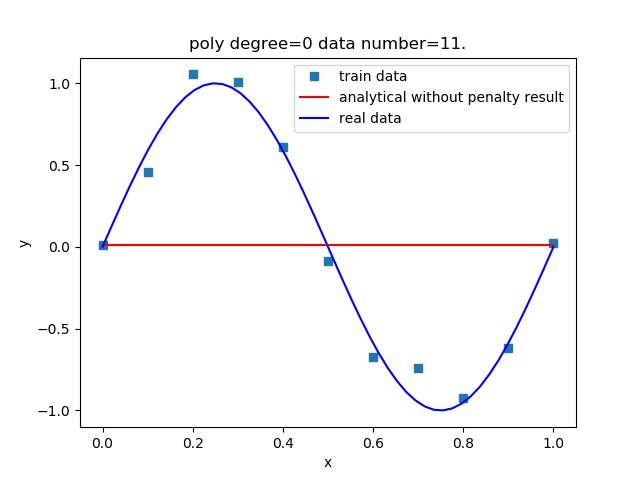
\includegraphics[width=.33\textwidth]{analyticalwithoutpenaltypolydegree=0datanumber=11.png}}\hfill
	\subfloat[poly degree = 1]{%
		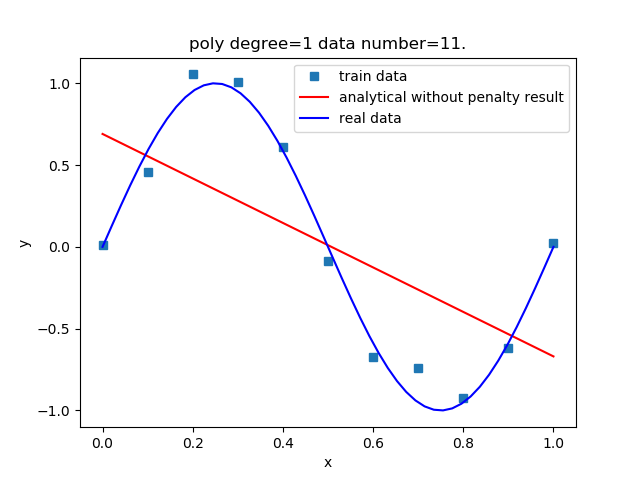
\includegraphics[width=.33\textwidth]{analyticalwithoutpenaltypolydegree=1datanumber=11.png}}\hfill
	\subfloat[poly degree = 2]{%
		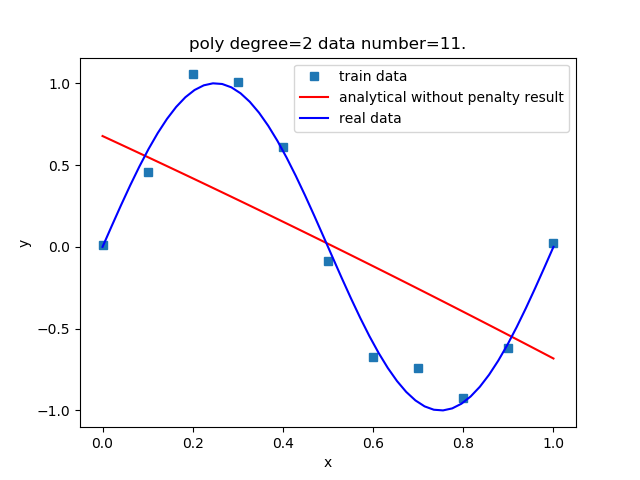
\includegraphics[width=.33\textwidth]{analyticalwithoutpenaltypolydegree=2datanumber=11.png}}\hfill
	\\
	\subfloat[poly degree = 3]{%
		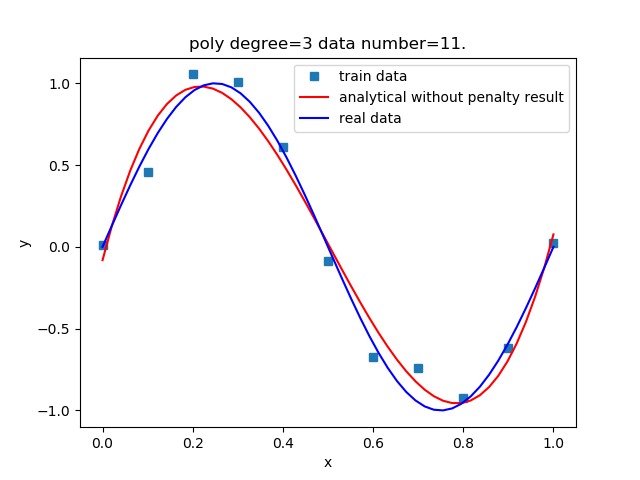
\includegraphics[width=.33\textwidth]{analyticalwithoutpenaltypolydegree=3datanumber=11.png}}\hfill
	\subfloat[poly degree = 4]{%
		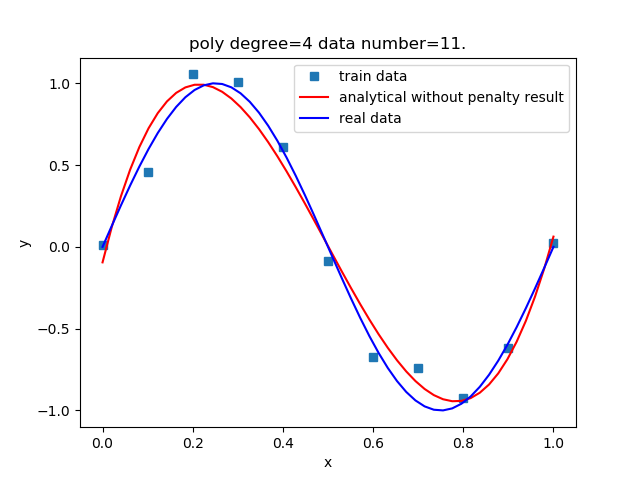
\includegraphics[width=.33\textwidth]{analyticalwithoutpenaltypolydegree=4datanumber=11.png}}\hfill
	\subfloat[poly degree = 5]{%
		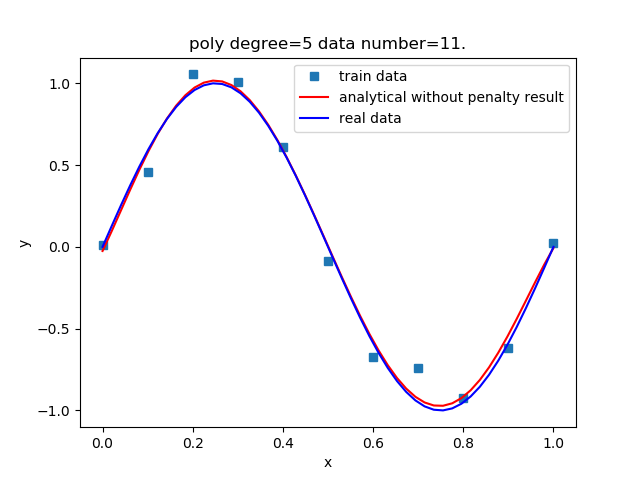
\includegraphics[width=.33\textwidth]{analyticalwithoutpenaltypolydegree=5datanumber=11.png}}\hfill
	\\
	\subfloat[poly degree = 6]{%
		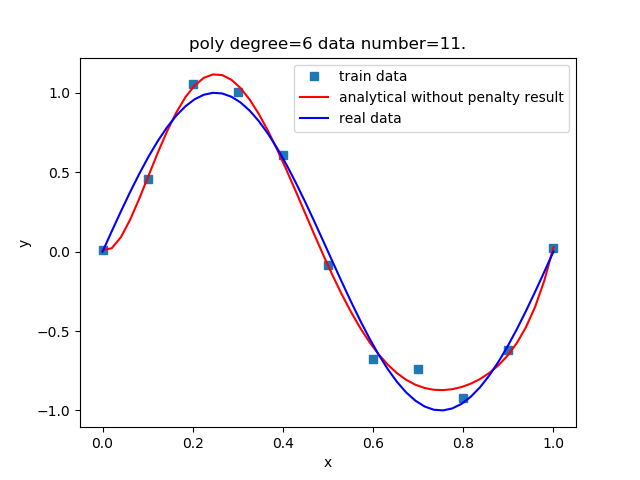
\includegraphics[width=.33\textwidth]{analyticalwithoutpenaltypolydegree=6datanumber=11.png}}\hfill
	\subfloat[poly degree = 7]{%
		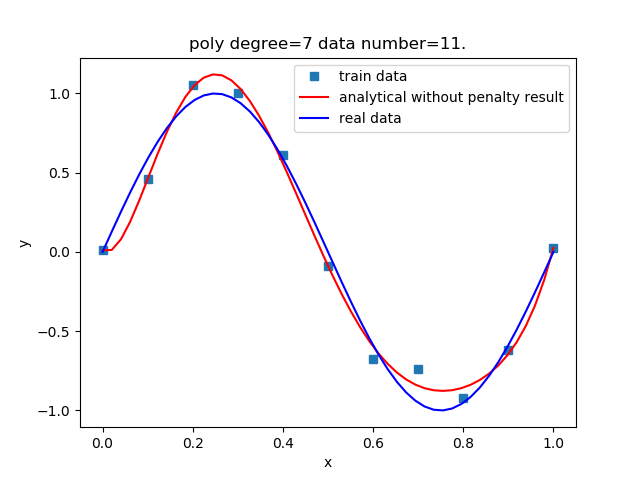
\includegraphics[width=.33\textwidth]{analyticalwithoutpenaltypolydegree=7datanumber=11.png}}\hfill
	\subfloat[poly degree = 8]{%
		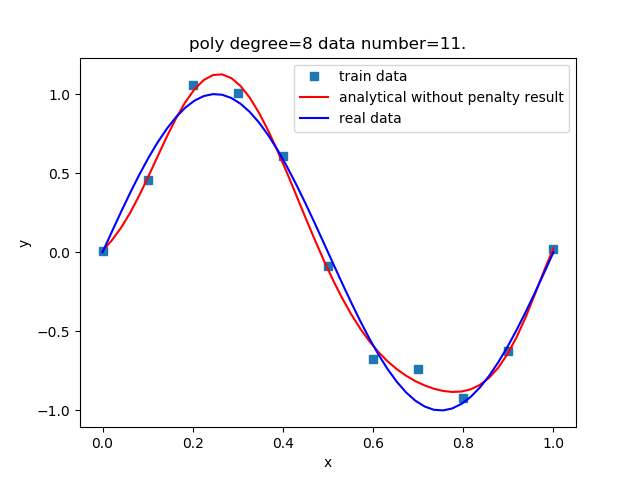
\includegraphics[width=.33\textwidth]{analyticalwithoutpenaltypolydegree=8datanumber=11.png}}\hfill
	\\
	\subfloat[poly degree = 9]{%
		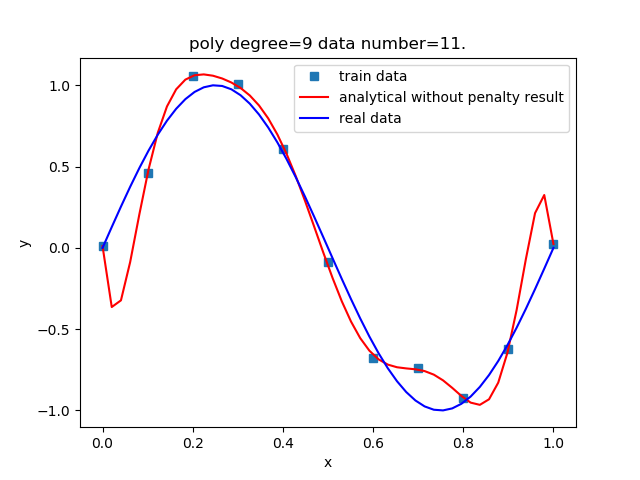
\includegraphics[width=.33\textwidth]{analyticalwithoutpenaltypolydegree=9datanumber=11.png}}
	\subfloat[poly degree = 10]{%
		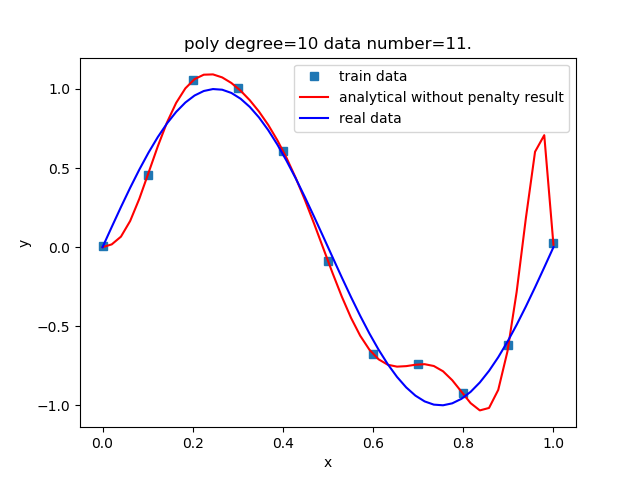
\includegraphics[width=.33\textwidth]{analyticalwithoutpenaltypolydegree=10datanumber=11.png}}	
	\caption{数据量为11时不同阶数不加惩罚项数值解法的拟合效果}\label{fig:analyticalwithoutpenalty}
\end{figure}

加惩罚项的数值解法拟合结果如图\ref{fig:analyticalwithpenalty}所示。

\begin{figure}[htb]
	\centering
	\subfloat[poly degree = 0]{%
		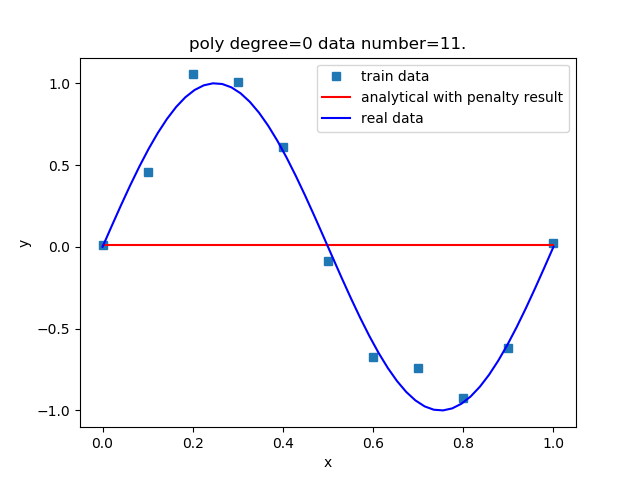
\includegraphics[width=.33\textwidth]{analyticalwithpenaltypolydegree=0datanumber=11.png}}\hfill
	\subfloat[poly degree = 1]{%
		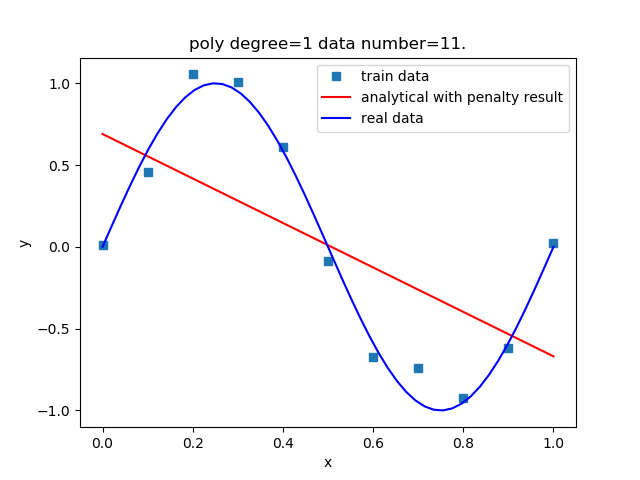
\includegraphics[width=.33\textwidth]{analyticalwithpenaltypolydegree=1datanumber=11.png}}\hfill
	\subfloat[poly degree = 2]{%
		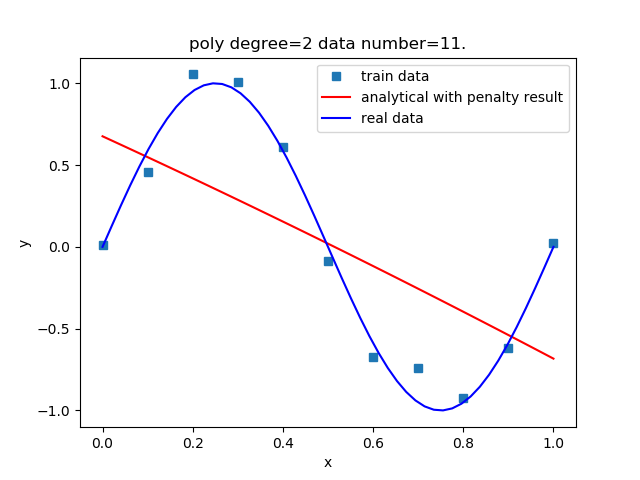
\includegraphics[width=.33\textwidth]{analyticalwithpenaltypolydegree=2datanumber=11.png}}\hfill
	\\
	\subfloat[poly degree = 3]{%
		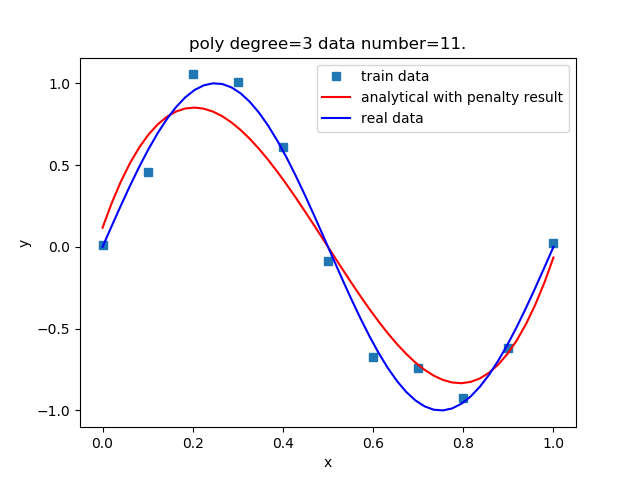
\includegraphics[width=.33\textwidth]{analyticalwithpenaltypolydegree=3datanumber=11.png}}\hfill
	\subfloat[poly degree = 4]{%
		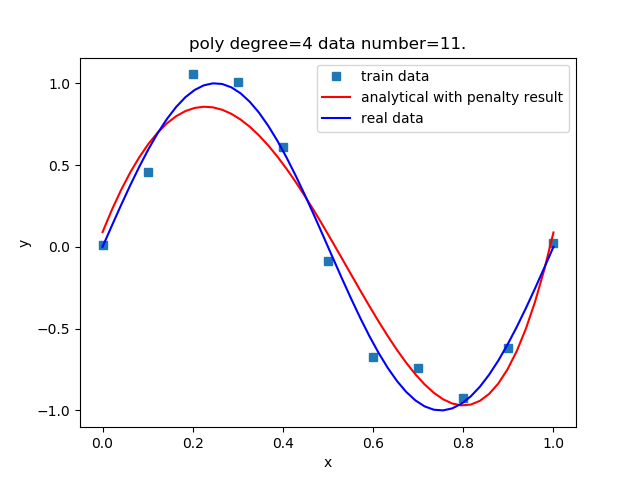
\includegraphics[width=.33\textwidth]{analyticalwithpenaltypolydegree=4datanumber=11.png}}\hfill
	\subfloat[poly degree = 5]{%
		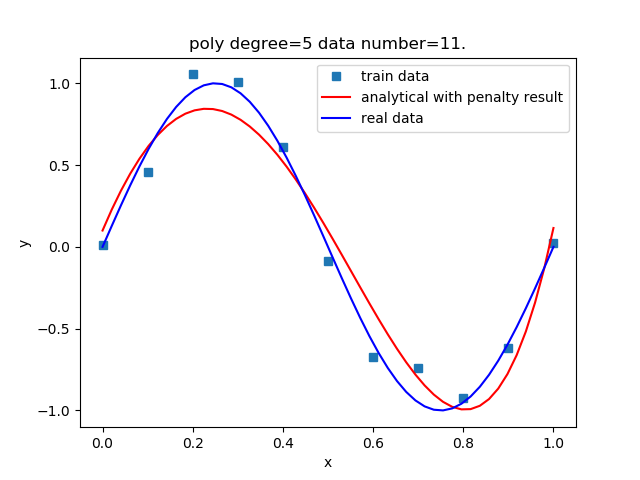
\includegraphics[width=.33\textwidth]{analyticalwithpenaltypolydegree=5datanumber=11.png}}\hfill
	\\
	\subfloat[poly degree = 6]{%
		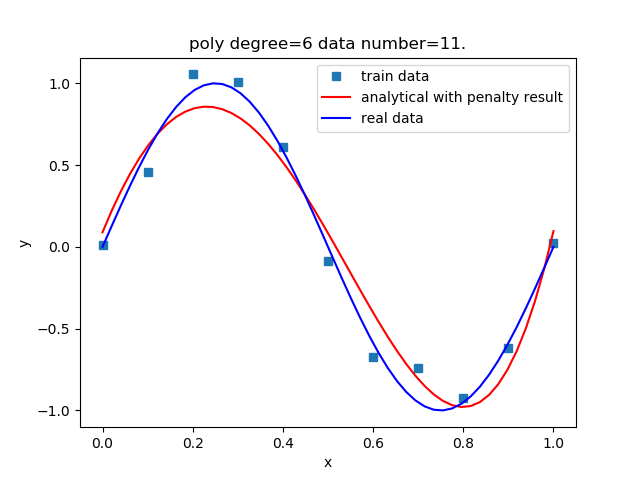
\includegraphics[width=.33\textwidth]{analyticalwithpenaltypolydegree=6datanumber=11.png}}\hfill
	\subfloat[poly degree = 7]{%
		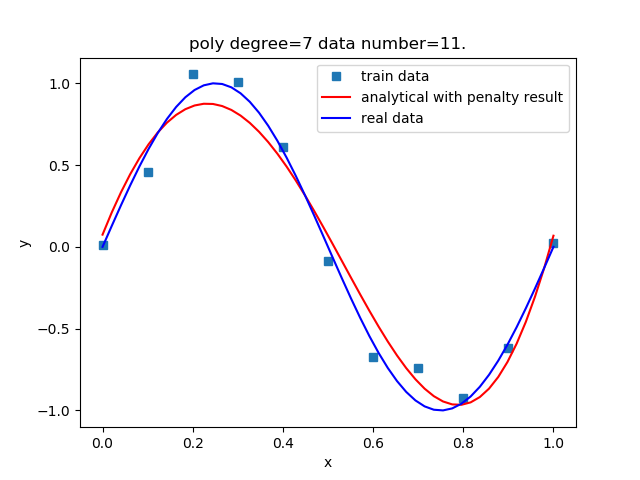
\includegraphics[width=.33\textwidth]{analyticalwithpenaltypolydegree=7datanumber=11.png}}\hfill
	\subfloat[poly degree = 8]{%
		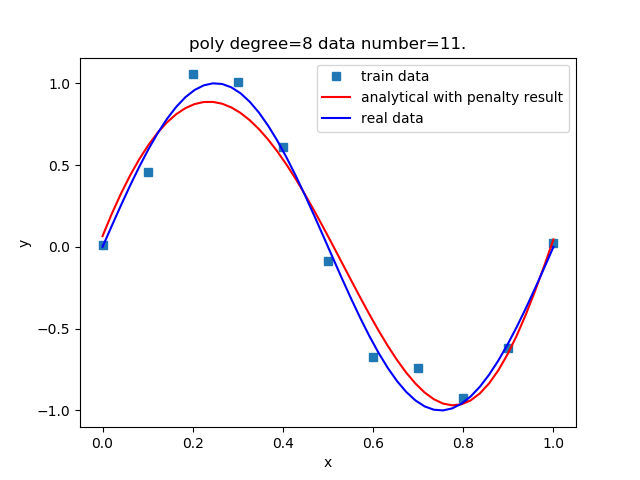
\includegraphics[width=.33\textwidth]{analyticalwithpenaltypolydegree=8datanumber=11.png}}\hfill
	\\
	\subfloat[poly degree = 9]{%
		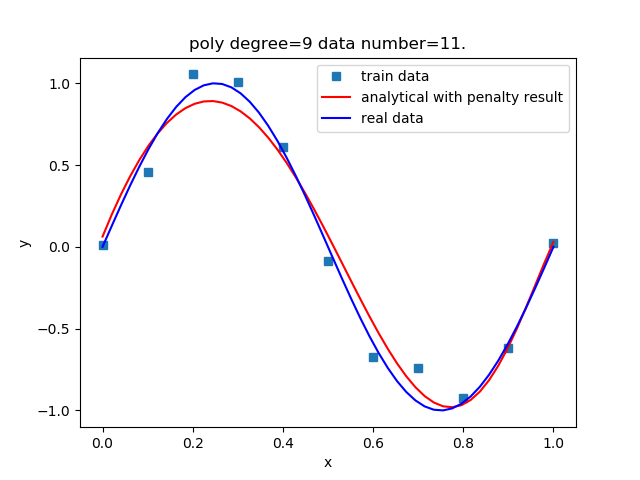
\includegraphics[width=.33\textwidth]{analyticalwithpenaltypolydegree=9datanumber=11.png}}
	\subfloat[poly degree = 10]{%
		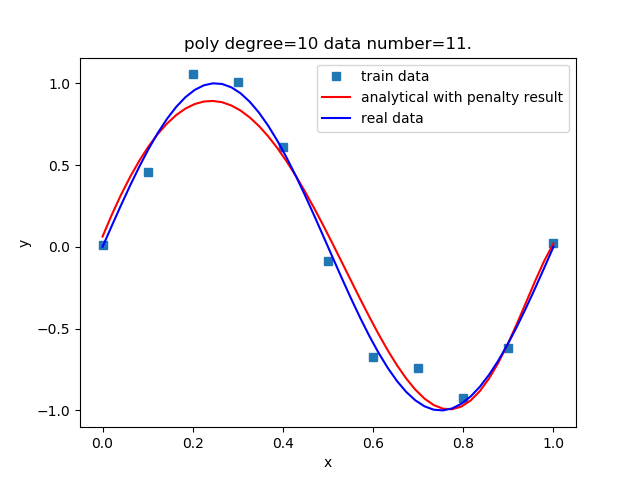
\includegraphics[width=.33\textwidth]{analyticalwithpenaltypolydegree=10datanumber=11.png}}	
	\caption{数据量为11时不同阶数加惩罚项数值解法的拟合效果}\label{fig:analyticalwithpenalty}
\end{figure}

\subsubsection{梯度下降法}

不加惩罚项的梯度下降法拟合结果如图\ref{fig:gradientdescentwithoutpenalty}所示。

\begin{figure}[htb]
	\centering
	\subfloat[poly degree = 0]{%
		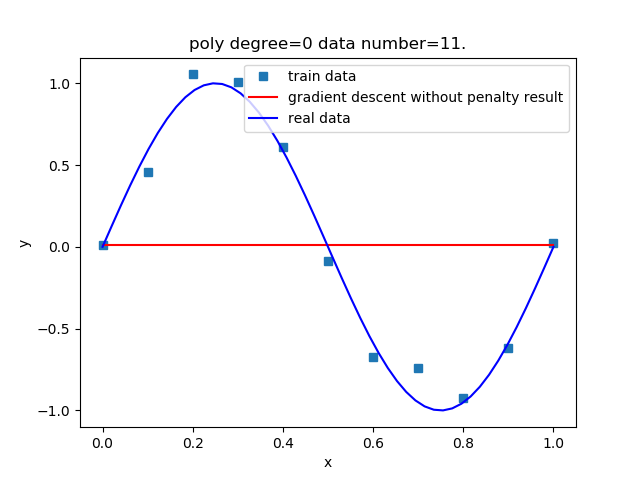
\includegraphics[width=.33\textwidth]{gradientdescentwithoutpenaltypolydegree=0datanumber=11.png}}\hfill
	\subfloat[poly degree = 1]{%
		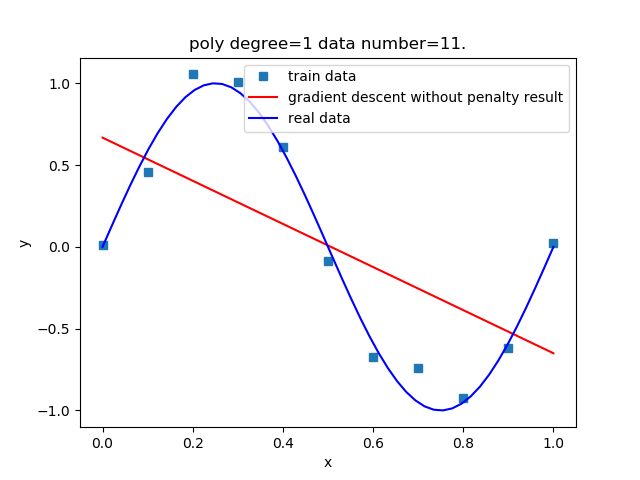
\includegraphics[width=.33\textwidth]{gradientdescentwithoutpenaltypolydegree=1datanumber=11.png}}\hfill
	\subfloat[poly degree = 2]{%
		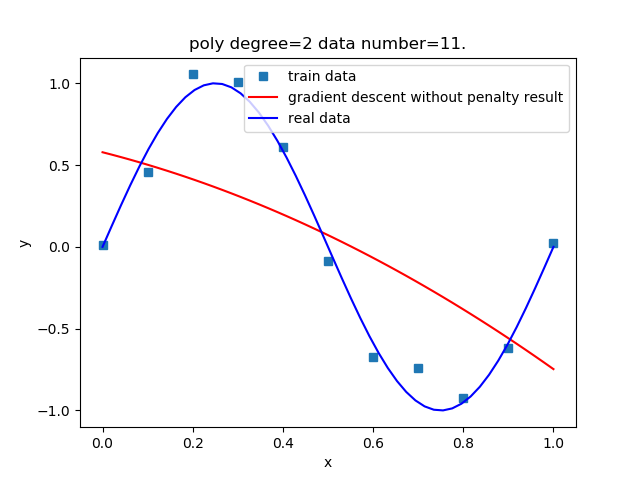
\includegraphics[width=.33\textwidth]{gradientdescentwithoutpenaltypolydegree=2datanumber=11.png}}\hfill
	\\
	\subfloat[poly degree = 3]{%
		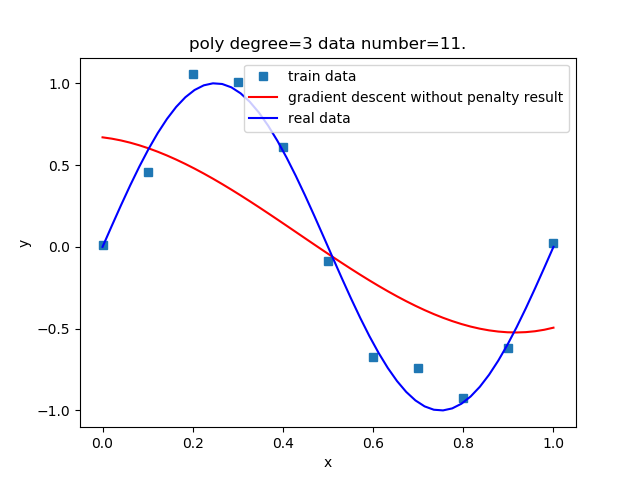
\includegraphics[width=.33\textwidth]{gradientdescentwithoutpenaltypolydegree=3datanumber=11.png}}\hfill
	\subfloat[poly degree = 4]{%
		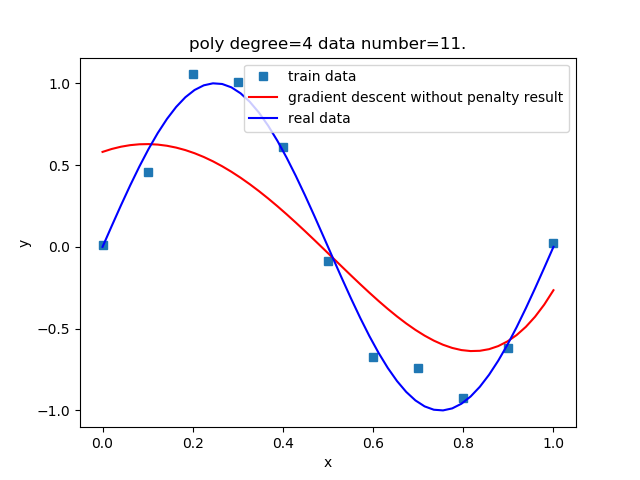
\includegraphics[width=.33\textwidth]{gradientdescentwithoutpenaltypolydegree=4datanumber=11.png}}\hfill
	\subfloat[poly degree = 5]{%
		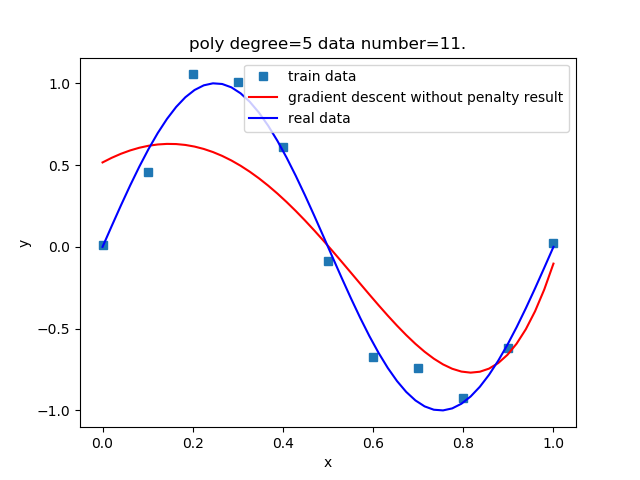
\includegraphics[width=.33\textwidth]{gradientdescentwithoutpenaltypolydegree=5datanumber=11.png}}\hfill
	\\
	\subfloat[poly degree = 6]{%
		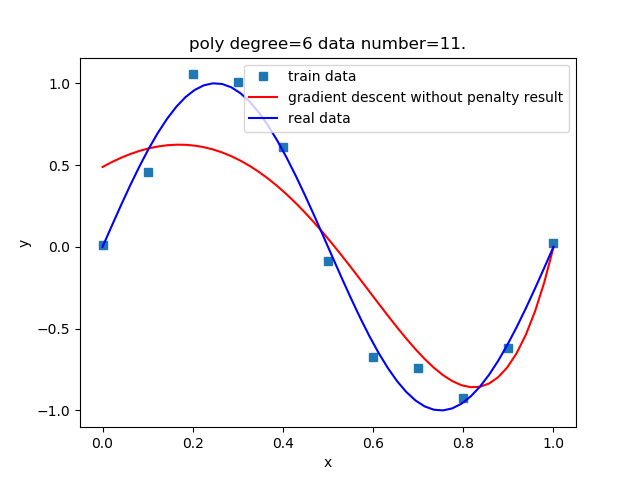
\includegraphics[width=.33\textwidth]{gradientdescentwithoutpenaltypolydegree=6datanumber=11.png}}\hfill
	\subfloat[poly degree = 7]{%
		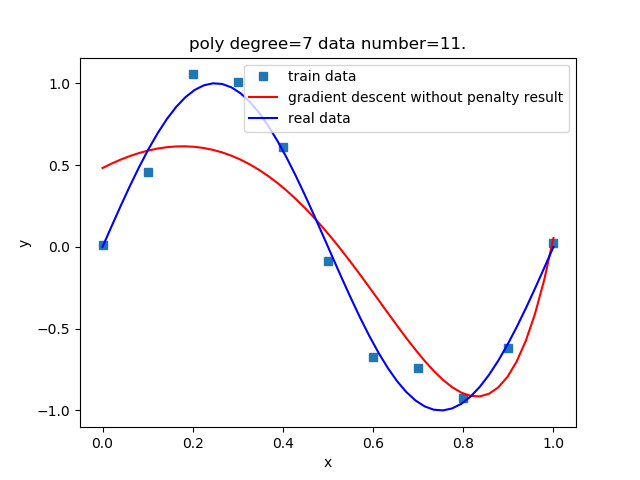
\includegraphics[width=.33\textwidth]{gradientdescentwithoutpenaltypolydegree=7datanumber=11.png}}\hfill
	\subfloat[poly degree = 8]{%
		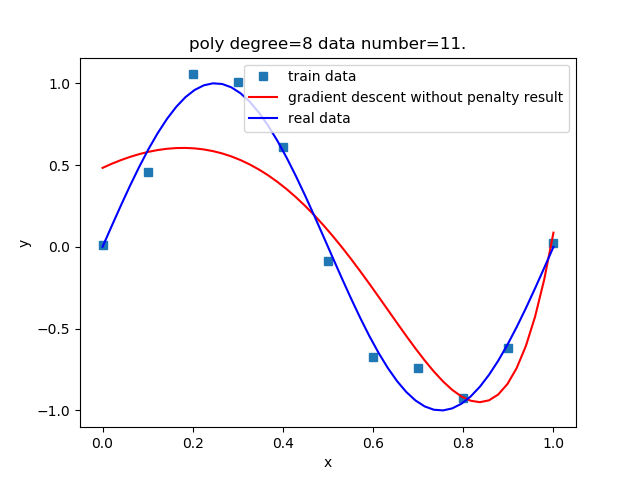
\includegraphics[width=.33\textwidth]{gradientdescentwithoutpenaltypolydegree=8datanumber=11.png}}\hfill
	\\
	\subfloat[poly degree = 9]{%
		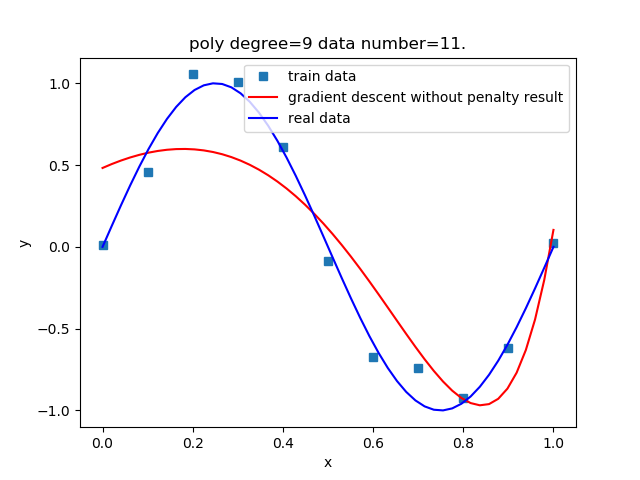
\includegraphics[width=.33\textwidth]{gradientdescentwithoutpenaltypolydegree=9datanumber=11.png}}
	\subfloat[poly degree = 10]{%
		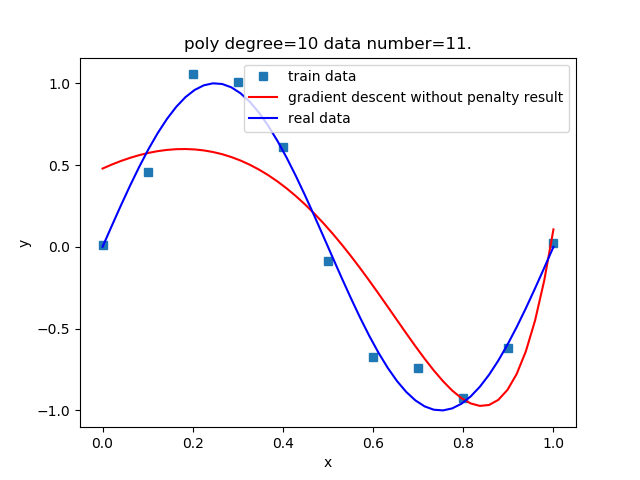
\includegraphics[width=.33\textwidth]{gradientdescentwithoutpenaltypolydegree=10datanumber=11.png}}	
	\caption{数据量为11时不同阶数不加惩罚项梯度下降法的拟合效果}\label{fig:gradientdescentwithoutpenalty}
\end{figure}

加惩罚项的梯度下降法拟合结果如图\ref{fig:gradientdescentwithpenalty}所示。

\begin{figure}[htb]
	\centering
	\subfloat[poly degree = 0]{%
		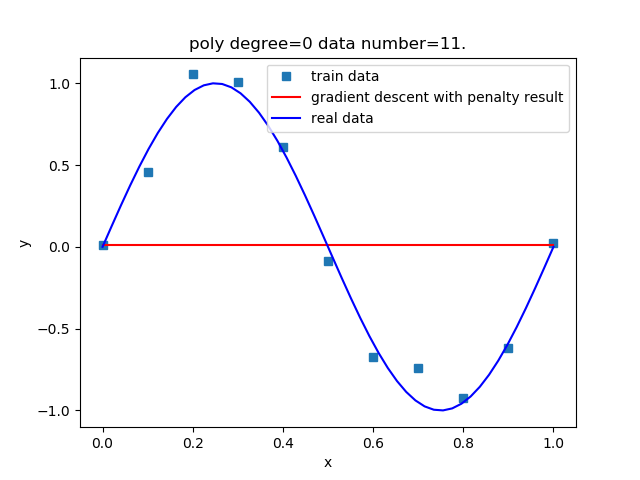
\includegraphics[width=.33\textwidth]{gradientdescentwithpenaltypolydegree=0datanumber=11.png}}\hfill
	\subfloat[poly degree = 1]{%
		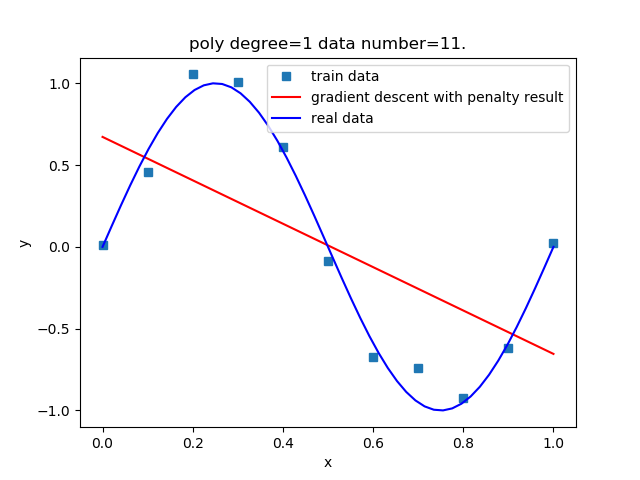
\includegraphics[width=.33\textwidth]{gradientdescentwithpenaltypolydegree=1datanumber=11.png}}\hfill
	\subfloat[poly degree = 2]{%
		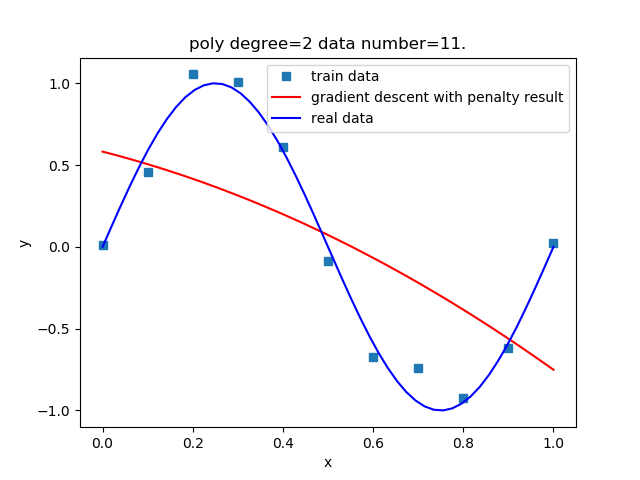
\includegraphics[width=.33\textwidth]{gradientdescentwithpenaltypolydegree=2datanumber=11.png}}\hfill
	\\
	\subfloat[poly degree = 3]{%
		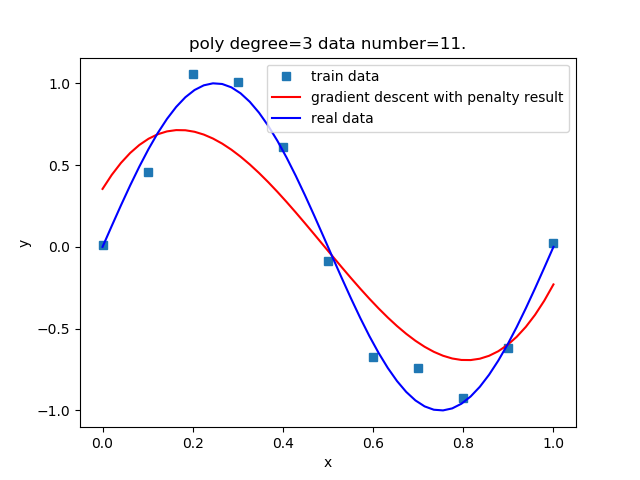
\includegraphics[width=.33\textwidth]{gradientdescentwithpenaltypolydegree=3datanumber=11.png}}\hfill
	\subfloat[poly degree = 4]{%
		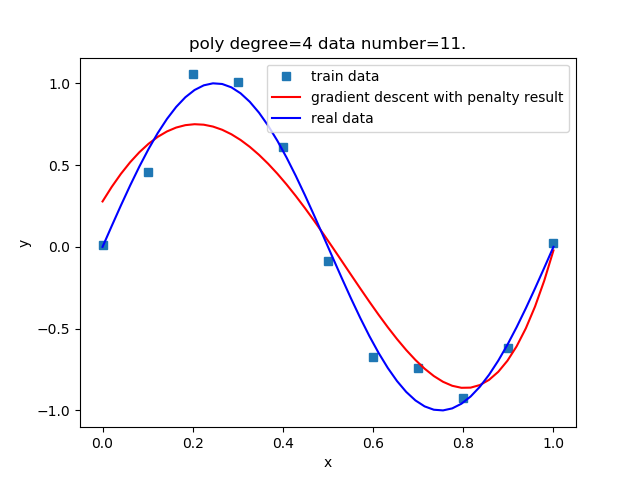
\includegraphics[width=.33\textwidth]{gradientdescentwithpenaltypolydegree=4datanumber=11.png}}\hfill
	\subfloat[poly degree = 5]{%
		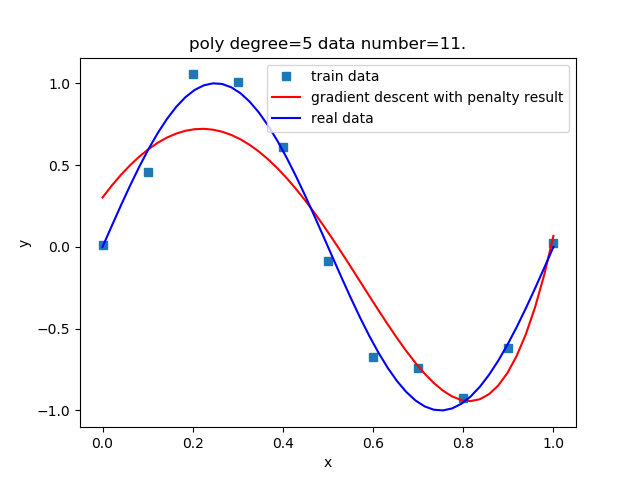
\includegraphics[width=.33\textwidth]{gradientdescentwithpenaltypolydegree=5datanumber=11.png}}\hfill
	\\
	\subfloat[poly degree = 6]{%
		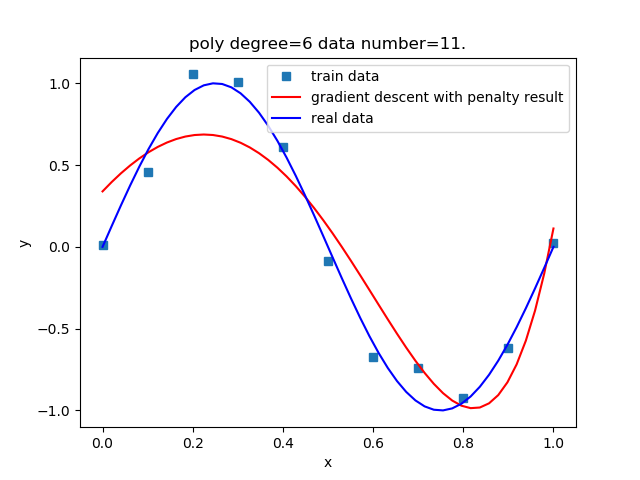
\includegraphics[width=.33\textwidth]{gradientdescentwithpenaltypolydegree=6datanumber=11.png}}\hfill
	\subfloat[poly degree = 7]{%
		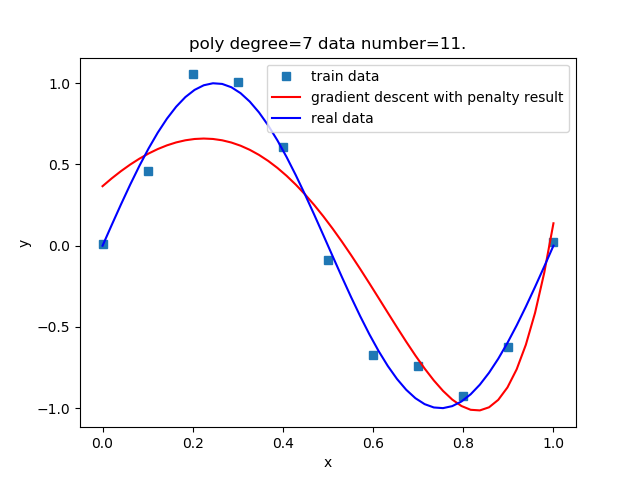
\includegraphics[width=.33\textwidth]{gradientdescentwithpenaltypolydegree=7datanumber=11.png}}\hfill
	\subfloat[poly degree = 8]{%
		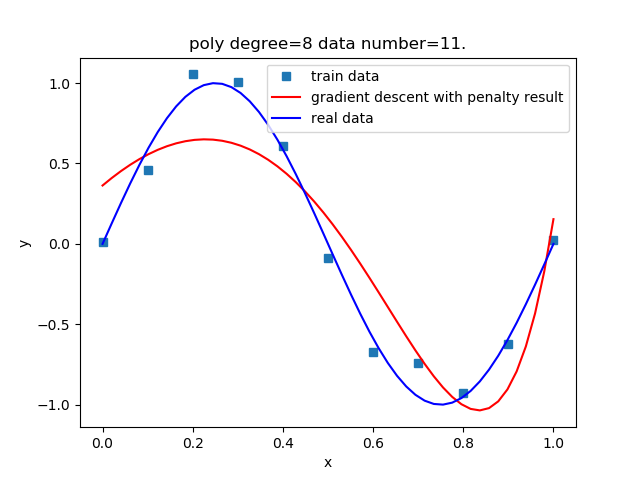
\includegraphics[width=.33\textwidth]{gradientdescentwithpenaltypolydegree=8datanumber=11.png}}\hfill
	\\
	\subfloat[poly degree = 9]{%
		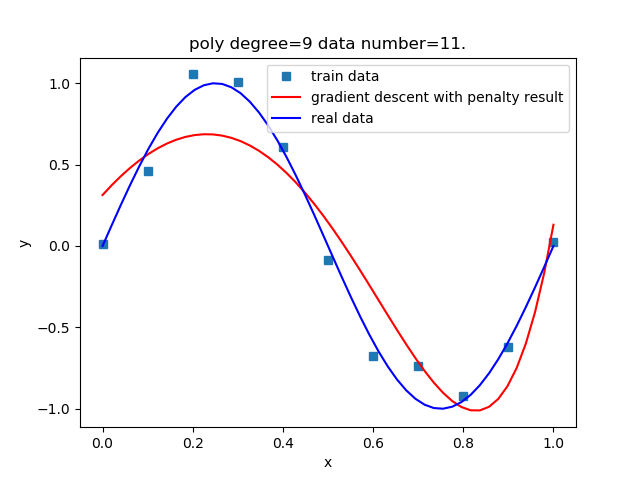
\includegraphics[width=.33\textwidth]{gradientdescentwithpenaltypolydegree=9datanumber=11.png}}
	\subfloat[poly degree = 10]{%
		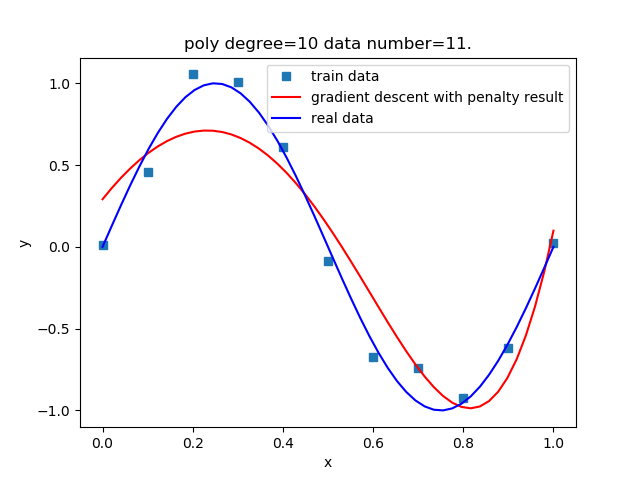
\includegraphics[width=.33\textwidth]{gradientdescentwithpenaltypolydegree=10datanumber=11.png}}	
	\caption{数据量为11时不同阶数加惩罚项梯度下降法的拟合效果}\label{fig:gradientdescentwithpenalty}
\end{figure}

\subsubsection{共轭梯度法}

不加惩罚项的共轭梯度法拟合结果如图\ref{fig:conjugategradientwithoutpenalty}所示。

\begin{figure}[htb]
	\centering
	\subfloat[poly degree = 0]{%
		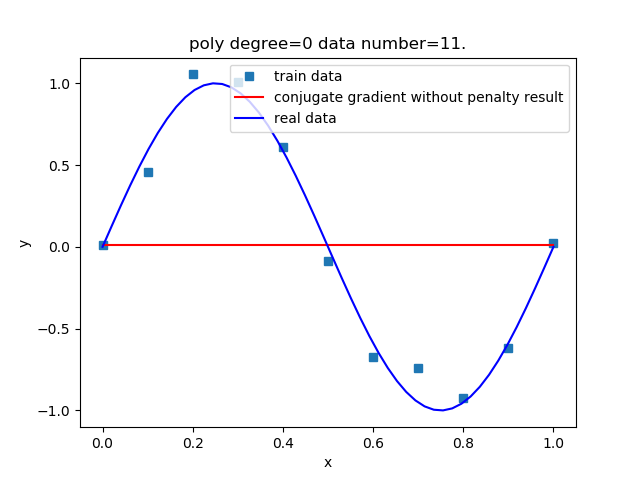
\includegraphics[width=.33\textwidth]{conjugategradientwithoutpenaltypolydegree=0datanumber=11.png}}\hfill
	\subfloat[poly degree = 1]{%
		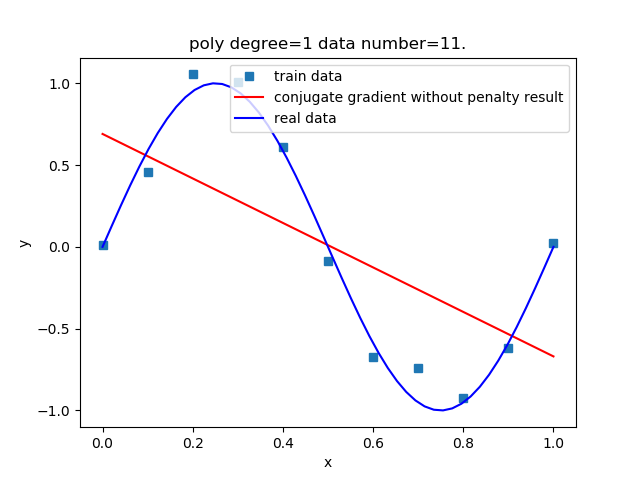
\includegraphics[width=.33\textwidth]{conjugategradientwithoutpenaltypolydegree=1datanumber=11.png}}\hfill
	\subfloat[poly degree = 2]{%
		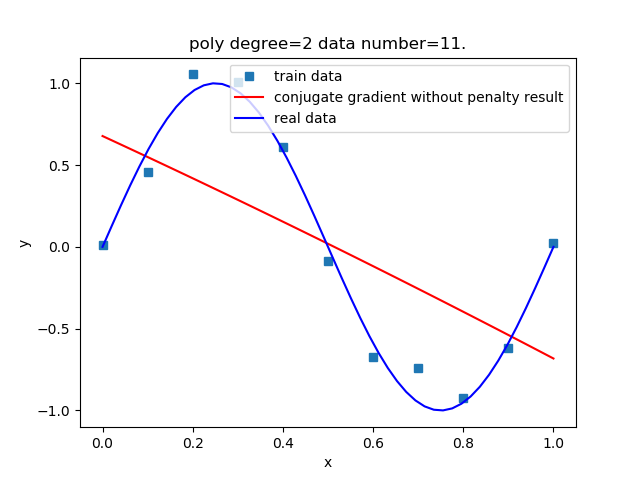
\includegraphics[width=.33\textwidth]{conjugategradientwithoutpenaltypolydegree=2datanumber=11.png}}\hfill
	\\
	\subfloat[poly degree = 3]{%
		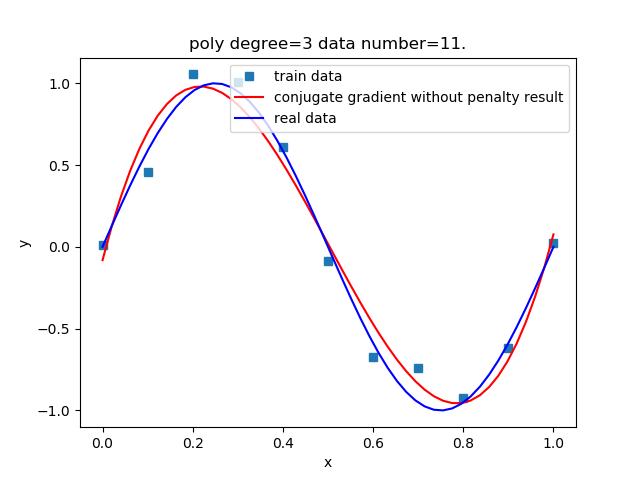
\includegraphics[width=.33\textwidth]{conjugategradientwithoutpenaltypolydegree=3datanumber=11.png}}\hfill
	\subfloat[poly degree = 4]{%
		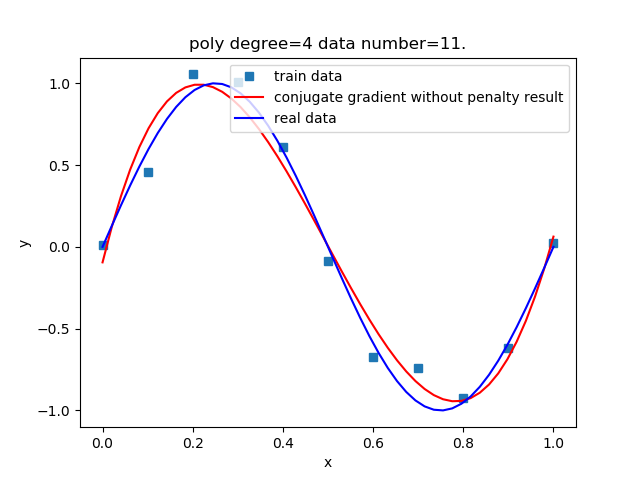
\includegraphics[width=.33\textwidth]{conjugategradientwithoutpenaltypolydegree=4datanumber=11.png}}\hfill
	\subfloat[poly degree = 5]{%
		\includegraphics[width=.33\textwidth]{conjugategradientwithoutpenaltypolydegree=5datanumber=11.png}}\hfill
	\\
	\subfloat[poly degree = 6]{%
		\includegraphics[width=.33\textwidth]{conjugategradientwithoutpenaltypolydegree=6datanumber=11.png}}\hfill
	\subfloat[poly degree = 7]{%
		\includegraphics[width=.33\textwidth]{conjugategradientwithoutpenaltypolydegree=7datanumber=11.png}}\hfill
	\subfloat[poly degree = 8]{%
		\includegraphics[width=.33\textwidth]{conjugategradientwithoutpenaltypolydegree=8datanumber=11.png}}\hfill
	\\
	\subfloat[poly degree = 9]{%
		\includegraphics[width=.33\textwidth]{conjugategradientwithoutpenaltypolydegree=9datanumber=11.png}}
	\subfloat[poly degree = 10]{%
		\includegraphics[width=.33\textwidth]{conjugategradientwithoutpenaltypolydegree=10datanumber=11.png}}	
	\caption{数据量为11时不同阶数不加惩罚项共轭梯度法的拟合效果}\label{fig:conjugategradientwithoutpenalty}
\end{figure}

加惩罚项的共轭梯度法拟合结果如图\ref{fig:conjugategradientwithpenalty}所示。

\begin{figure}[htb]
	\centering
	\subfloat[poly degree = 0]{%
		\includegraphics[width=.33\textwidth]{conjugategradientwithpenaltypolydegree=0datanumber=11.png}}\hfill
	\subfloat[poly degree = 1]{%
		\includegraphics[width=.33\textwidth]{conjugategradientwithpenaltypolydegree=1datanumber=11.png}}\hfill
	\subfloat[poly degree = 2]{%
		\includegraphics[width=.33\textwidth]{conjugategradientwithpenaltypolydegree=2datanumber=11.png}}\hfill
	\\
	\subfloat[poly degree = 3]{%
		\includegraphics[width=.33\textwidth]{conjugategradientwithpenaltypolydegree=3datanumber=11.png}}\hfill
	\subfloat[poly degree = 4]{%
		\includegraphics[width=.33\textwidth]{conjugategradientwithpenaltypolydegree=4datanumber=11.png}}\hfill
	\subfloat[poly degree = 5]{%
		\includegraphics[width=.33\textwidth]{conjugategradientwithpenaltypolydegree=5datanumber=11.png}}\hfill
	\\
	\subfloat[poly degree = 6]{%
		\includegraphics[width=.33\textwidth]{conjugategradientwithpenaltypolydegree=6datanumber=11.png}}\hfill
	\subfloat[poly degree = 7]{%
		\includegraphics[width=.33\textwidth]{conjugategradientwithpenaltypolydegree=7datanumber=11.png}}\hfill
	\subfloat[poly degree = 8]{%
		\includegraphics[width=.33\textwidth]{conjugategradientwithpenaltypolydegree=8datanumber=11.png}}\hfill
	\\
	\subfloat[poly degree = 9]{%
		\includegraphics[width=.33\textwidth]{conjugategradientwithpenaltypolydegree=9datanumber=11.png}}
	\subfloat[poly degree = 10]{%
		\includegraphics[width=.33\textwidth]{conjugategradientwithpenaltypolydegree=10datanumber=11.png}}	
	\caption{数据量为11时不同阶数加惩罚项共轭梯度法的拟合效果}\label{fig:conjugategradientwithpenalty}
\end{figure}



\subsection{数据量为100时不同阶数不同方法的拟合效果}

\subsubsection{数值解法}

不加惩罚项的数值解法拟合结果如图\ref{fig:100analyticalwithoutpenalty}所示。

\begin{figure}[htb]
	\centering
	\subfloat[poly degree = 0]{%
		\includegraphics[width=.33\textwidth]{analyticalwithoutpenaltypolydegree=0datanumber=100.png}}\hfill
	\subfloat[poly degree = 1]{%
		\includegraphics[width=.33\textwidth]{analyticalwithoutpenaltypolydegree=1datanumber=100.png}}\hfill
	\subfloat[poly degree = 2]{%
		\includegraphics[width=.33\textwidth]{analyticalwithoutpenaltypolydegree=2datanumber=100.png}}\hfill
	\\
	\subfloat[poly degree = 3]{%
		\includegraphics[width=.33\textwidth]{analyticalwithoutpenaltypolydegree=3datanumber=100.png}}\hfill
	\subfloat[poly degree = 4]{%
		\includegraphics[width=.33\textwidth]{analyticalwithoutpenaltypolydegree=4datanumber=100.png}}\hfill
	\subfloat[poly degree = 5]{%
		\includegraphics[width=.33\textwidth]{analyticalwithoutpenaltypolydegree=5datanumber=100.png}}\hfill
	\\
	\subfloat[poly degree = 6]{%
		\includegraphics[width=.33\textwidth]{analyticalwithoutpenaltypolydegree=6datanumber=100.png}}\hfill
	\subfloat[poly degree = 7]{%
		\includegraphics[width=.33\textwidth]{analyticalwithoutpenaltypolydegree=7datanumber=100.png}}\hfill
	\subfloat[poly degree = 8]{%
		\includegraphics[width=.33\textwidth]{analyticalwithoutpenaltypolydegree=8datanumber=100.png}}\hfill
	\\
	\subfloat[poly degree = 9]{%
		\includegraphics[width=.33\textwidth]{analyticalwithoutpenaltypolydegree=9datanumber=100.png}}
	\subfloat[poly degree = 10]{%
		\includegraphics[width=.33\textwidth]{analyticalwithoutpenaltypolydegree=10datanumber=100.png}}	
	\caption{数据量为11时不同阶数不加惩罚项数值解法的拟合效果}\label{fig:100analyticalwithoutpenalty}
\end{figure}

加惩罚项的数值解法拟合结果如图\ref{fig:100analyticalwithpenalty}所示。

\begin{figure}[htb]
	\centering
	\subfloat[poly degree = 0]{%
		\includegraphics[width=.33\textwidth]{analyticalwithpenaltypolydegree=0datanumber=100.png}}\hfill
	\subfloat[poly degree = 1]{%
		\includegraphics[width=.33\textwidth]{analyticalwithpenaltypolydegree=1datanumber=100.png}}\hfill
	\subfloat[poly degree = 2]{%
		\includegraphics[width=.33\textwidth]{analyticalwithpenaltypolydegree=2datanumber=100.png}}\hfill
	\\
	\subfloat[poly degree = 3]{%
		\includegraphics[width=.33\textwidth]{analyticalwithpenaltypolydegree=3datanumber=100.png}}\hfill
	\subfloat[poly degree = 4]{%
		\includegraphics[width=.33\textwidth]{analyticalwithpenaltypolydegree=4datanumber=100.png}}\hfill
	\subfloat[poly degree = 5]{%
		\includegraphics[width=.33\textwidth]{analyticalwithpenaltypolydegree=5datanumber=100.png}}\hfill
	\\
	\subfloat[poly degree = 6]{%
		\includegraphics[width=.33\textwidth]{analyticalwithpenaltypolydegree=6datanumber=100.png}}\hfill
	\subfloat[poly degree = 7]{%
		\includegraphics[width=.33\textwidth]{analyticalwithpenaltypolydegree=7datanumber=100.png}}\hfill
	\subfloat[poly degree = 8]{%
		\includegraphics[width=.33\textwidth]{analyticalwithpenaltypolydegree=8datanumber=100.png}}\hfill
	\\
	\subfloat[poly degree = 9]{%
		\includegraphics[width=.33\textwidth]{analyticalwithpenaltypolydegree=9datanumber=100.png}}
	\subfloat[poly degree = 10]{%
		\includegraphics[width=.33\textwidth]{analyticalwithpenaltypolydegree=10datanumber=100.png}}	
	\caption{数据量为100时不同阶数加惩罚项数值解法的拟合效果}\label{fig:100analyticalwithpenalty}
\end{figure}

\subsubsection{梯度下降法}

不加惩罚项的梯度下降法拟合结果如图\ref{fig:100gradientdescentwithoutpenalty}所示。

\begin{figure}[htb]
	\centering
	\subfloat[poly degree = 0]{%
		\includegraphics[width=.33\textwidth]{gradientdescentwithoutpenaltypolydegree=0datanumber=100.png}}\hfill
	\subfloat[poly degree = 1]{%
		\includegraphics[width=.33\textwidth]{gradientdescentwithoutpenaltypolydegree=1datanumber=100.png}}\hfill
	\subfloat[poly degree = 2]{%
		\includegraphics[width=.33\textwidth]{gradientdescentwithoutpenaltypolydegree=2datanumber=100.png}}\hfill
	\\
	\subfloat[poly degree = 3]{%
		\includegraphics[width=.33\textwidth]{gradientdescentwithoutpenaltypolydegree=3datanumber=100.png}}\hfill
	\subfloat[poly degree = 4]{%
		\includegraphics[width=.33\textwidth]{gradientdescentwithoutpenaltypolydegree=4datanumber=100.png}}\hfill
	\subfloat[poly degree = 5]{%
		\includegraphics[width=.33\textwidth]{gradientdescentwithoutpenaltypolydegree=5datanumber=100.png}}\hfill
	\\
	\subfloat[poly degree = 6]{%
		\includegraphics[width=.33\textwidth]{gradientdescentwithoutpenaltypolydegree=6datanumber=100.png}}\hfill
	\subfloat[poly degree = 7]{%
		\includegraphics[width=.33\textwidth]{gradientdescentwithoutpenaltypolydegree=7datanumber=100.png}}\hfill
	\subfloat[poly degree = 8]{%
		\includegraphics[width=.33\textwidth]{gradientdescentwithoutpenaltypolydegree=8datanumber=100.png}}\hfill
	\\
	\subfloat[poly degree = 9]{%
		\includegraphics[width=.33\textwidth]{gradientdescentwithoutpenaltypolydegree=9datanumber=100.png}}
	\subfloat[poly degree = 10]{%
		\includegraphics[width=.33\textwidth]{gradientdescentwithoutpenaltypolydegree=10datanumber=100.png}}	
	\caption{数据量为100时不同阶数不加惩罚项梯度下降法的拟合效果}\label{fig:100gradientdescentwithoutpenalty}
\end{figure}

加惩罚项的梯度下降法拟合结果如图\ref{fig:100gradientdescentwithpenalty}所示。

\begin{figure}[htb]
	\centering
	\subfloat[poly degree = 0]{%
		\includegraphics[width=.33\textwidth]{gradientdescentwithpenaltypolydegree=0datanumber=100.png}}\hfill
	\subfloat[poly degree = 1]{%
		\includegraphics[width=.33\textwidth]{gradientdescentwithpenaltypolydegree=1datanumber=100.png}}\hfill
	\subfloat[poly degree = 2]{%
		\includegraphics[width=.33\textwidth]{gradientdescentwithpenaltypolydegree=2datanumber=100.png}}\hfill
	\\
	\subfloat[poly degree = 3]{%
		\includegraphics[width=.33\textwidth]{gradientdescentwithpenaltypolydegree=3datanumber=100.png}}\hfill
	\subfloat[poly degree = 4]{%
		\includegraphics[width=.33\textwidth]{gradientdescentwithpenaltypolydegree=4datanumber=100.png}}\hfill
	\subfloat[poly degree = 5]{%
		\includegraphics[width=.33\textwidth]{gradientdescentwithpenaltypolydegree=5datanumber=100.png}}\hfill
	\\
	\subfloat[poly degree = 6]{%
		\includegraphics[width=.33\textwidth]{gradientdescentwithpenaltypolydegree=6datanumber=100.png}}\hfill
	\subfloat[poly degree = 7]{%
		\includegraphics[width=.33\textwidth]{gradientdescentwithpenaltypolydegree=7datanumber=100.png}}\hfill
	\subfloat[poly degree = 8]{%
		\includegraphics[width=.33\textwidth]{gradientdescentwithpenaltypolydegree=8datanumber=100.png}}\hfill
	\\
	\subfloat[poly degree = 9]{%
		\includegraphics[width=.33\textwidth]{gradientdescentwithpenaltypolydegree=9datanumber=100.png}}
	\subfloat[poly degree = 10]{%
		\includegraphics[width=.33\textwidth]{gradientdescentwithpenaltypolydegree=10datanumber=100.png}}	
	\caption{数据量为100时不同阶数加惩罚项梯度下降法的拟合效果}\label{fig:100gradientdescentwithpenalty}
\end{figure}

\subsubsection{共轭梯度法}

不加惩罚项的共轭梯度法拟合结果如图\ref{fig:100conjugategradientwithoutpenalty}所示。

\begin{figure}[htb]
	\centering
	\subfloat[poly degree = 0]{%
		\includegraphics[width=.33\textwidth]{conjugategradientwithoutpenaltypolydegree=0datanumber=100.png}}\hfill
	\subfloat[poly degree = 1]{%
		\includegraphics[width=.33\textwidth]{conjugategradientwithoutpenaltypolydegree=1datanumber=100.png}}\hfill
	\subfloat[poly degree = 2]{%
		\includegraphics[width=.33\textwidth]{conjugategradientwithoutpenaltypolydegree=2datanumber=100.png}}\hfill
	\\
	\subfloat[poly degree = 3]{%
		\includegraphics[width=.33\textwidth]{conjugategradientwithoutpenaltypolydegree=3datanumber=100.png}}\hfill
	\subfloat[poly degree = 4]{%
		\includegraphics[width=.33\textwidth]{conjugategradientwithoutpenaltypolydegree=4datanumber=100.png}}\hfill
	\subfloat[poly degree = 5]{%
		\includegraphics[width=.33\textwidth]{conjugategradientwithoutpenaltypolydegree=5datanumber=100.png}}\hfill
	\\
	\subfloat[poly degree = 6]{%
		\includegraphics[width=.33\textwidth]{conjugategradientwithoutpenaltypolydegree=6datanumber=100.png}}\hfill
	\subfloat[poly degree = 7]{%
		\includegraphics[width=.33\textwidth]{conjugategradientwithoutpenaltypolydegree=7datanumber=100.png}}\hfill
	\subfloat[poly degree = 8]{%
		\includegraphics[width=.33\textwidth]{conjugategradientwithoutpenaltypolydegree=8datanumber=100.png}}\hfill
	\\
	\subfloat[poly degree = 9]{%
		\includegraphics[width=.33\textwidth]{conjugategradientwithoutpenaltypolydegree=9datanumber=100.png}}
	\subfloat[poly degree = 10]{%
		\includegraphics[width=.33\textwidth]{conjugategradientwithoutpenaltypolydegree=10datanumber=100.png}}	
	\caption{数据量为100时不同阶数不加惩罚项共轭梯度法的拟合效果}\label{fig:100conjugategradientwithoutpenalty}
\end{figure}

加惩罚项的共轭梯度法拟合结果如图\ref{fig:100conjugategradientwithpenalty}所示。

\begin{figure}[htb]
	\centering
	\subfloat[poly degree = 0]{%
		\includegraphics[width=.33\textwidth]{conjugategradientwithpenaltypolydegree=0datanumber=100.png}}\hfill
	\subfloat[poly degree = 1]{%
		\includegraphics[width=.33\textwidth]{conjugategradientwithpenaltypolydegree=1datanumber=100.png}}\hfill
	\subfloat[poly degree = 2]{%
		\includegraphics[width=.33\textwidth]{conjugategradientwithpenaltypolydegree=2datanumber=100.png}}\hfill
	\\
	\subfloat[poly degree = 3]{%
		\includegraphics[width=.33\textwidth]{conjugategradientwithpenaltypolydegree=3datanumber=100.png}}\hfill
	\subfloat[poly degree = 4]{%
		\includegraphics[width=.33\textwidth]{conjugategradientwithpenaltypolydegree=4datanumber=100.png}}\hfill
	\subfloat[poly degree = 5]{%
		\includegraphics[width=.33\textwidth]{conjugategradientwithpenaltypolydegree=5datanumber=100.png}}\hfill
	\\
	\subfloat[poly degree = 6]{%
		\includegraphics[width=.33\textwidth]{conjugategradientwithpenaltypolydegree=6datanumber=100.png}}\hfill
	\subfloat[poly degree = 7]{%
		\includegraphics[width=.33\textwidth]{conjugategradientwithpenaltypolydegree=7datanumber=100.png}}\hfill
	\subfloat[poly degree = 8]{%
		\includegraphics[width=.33\textwidth]{conjugategradientwithpenaltypolydegree=8datanumber=100.png}}\hfill
	\\
	\subfloat[poly degree = 9]{%
		\includegraphics[width=.33\textwidth]{conjugategradientwithpenaltypolydegree=9datanumber=100.png}}
	\subfloat[poly degree = 10]{%
		\includegraphics[width=.33\textwidth]{conjugategradientwithpenaltypolydegree=10datanumber=100.png}}	
	\caption{数据量为100时不同阶数加惩罚项共轭梯度法的拟合效果}\label{fig:100conjugategradientwithpenalty}
\end{figure}

\subsection{训练集与测试集的损失函数随阶数的变化}

当训练集的数量为11时,训练集与测试集的损失函数随阶数的变化如图\ref{fig:loss11}所示。
\begin{figure}
	\centering
	\includegraphics[width=0.6\linewidth]{lossofdifferentpolydegree,datanumber=11.png}
	\caption{训练集数量为11时,训练集与测试集的损失函数随阶数的变化}\label{fig:loss11}
\end{figure}


当训练集的数量为100时,训练集与测试集的损失函数随阶数的变化如图\ref{fig:loss100}所示。
\begin{figure}
	\centering
	\includegraphics[width=0.6\linewidth]{lossofdifferentpolydegree,datanumber=100.png}
	\caption{训练集数量为100时,训练集与测试集的损失函数随阶数的变化}\label{fig:loss100}
\end{figure}


%\begin{figure}[htb]
%	\centering
%	\subfloat[评级A企业贷款年利率和客户流失率关系]{%
%		\includegraphics[width=.33\textwidth]{2}}\hfill
%	\subfloat[评级B企业贷款年利率和客户流失率关系]{%
%		\includegraphics[width=.33\textwidth]{3}}\hfill
%	\subfloat[评级C企业贷款年利率和客户流失率关系]{%
%		\includegraphics[width=.33\textwidth]{4}}
%	\caption{不同信誉评级的企业贷款年利率和客户流失率关系图示}\label{fig:churn_rate}
%\end{figure}

%\section{操作方法和实验步骤}
%\subsection{传输函数}
%对差分方程进行处理,求出传输函数表达式.
%\subsection{零极点分布图}
%在此基础上,使用Matlab中的zplane函数进一步画出在不同a取值情况下的零极点分布图.
%\subsection{幅频响应}
%之后使用freqz函数画出不同a取值情况下的频率响应图像.
%
%\section{实验数据记录和处理}
%\subsection{传输函数}
%根据差分方程,传输函数如下:
%$$H(z) = \frac{Y(z)}{X(z)} = \frac{z^2}{z^2-(0.5+a)z+0.5a}$$
%\subsection{零极点分布图}
%a = 0.8,0.9,1.1时,系统的零极点分布图及程序如下:
%\begin{enumerate}
%  \item 图像
%        \begin{center}
%          \includegraphics[width=0.6\linewidth]{01.jpg}
%        \end{center}
%  \item 代码
%        \lstinputlisting[language=MATLAB]{code/do.m}
%\end{enumerate}
%
%\subsection{频率响应}
%a = 0.8,0.9,1.0,1.1时,系统的频率响应函数图形及程序如下:
%\begin{enumerate}
%  \item 图像
%        \begin{center}
%          \includegraphics[width=0.6\linewidth]{02-1.jpg}
%        \end{center}
%  \item 代码
%        \lstinputlisting[language=MATLAB]{code/next.m}
%\end{enumerate}

\section{实验结果分析}

根据实验结果,使用多项式对正弦函数$f\left(x\right) = \sin \left(2\pi x\right)$进行拟合时,多项式的次数越高,其拟合能力越强,在数据量为11且不加入惩罚项的情况下,次数较高的多项式出现了过拟合的现象。形成过拟合的主要原因是样本数量过少,而多项式次数过高会导致模型学习能力过强,模型拟合结果过分依赖数据量很少的数据集,而太少的样本存在一定偶然性,这种强拟合能力将并不具有普遍性的特征训练进了模型,从而无法拟合出正弦曲线。在数据集为100且不加入惩罚项的情况下,次数相对于100来说很低,所以并未出现过拟合的现象。但是在数据量为11且加入惩罚项的情况下,次数高的多项式也能减小过拟合现象。

因此,为了减小过拟合现象,可以增加惩罚项或增加数据量。根据实验结果,在目标函数中加入参数的惩罚项后,过拟合现象得到明显改善。这是由于参数增多时,往往具有较大的绝对值,加入正则项可以有效地降低参数的绝对值,从而使模型复杂度与问题匹配。但是当样本足够多时,惩罚项相对于数据就影响不大了。当惩罚项过小时,过拟合现象并没有明显的改善,惩罚项过大时,会出现欠拟合现象。增加数据量可以避免因为数据量较少而产生的随机误差,避免随机误差被当做数据特征被学习进模型中。

图片\ref{fig:loss11}与图片\ref{fig:loss100}也表明,在训练集的数据令较少的情况下,模型出现了过拟合的现象,尽管在训练集的损失函数达到了很小,但是测试集的损失函数也变得很大。当训练数据集的数量是100时,多项式阶数为10时也没有出现过拟合现象,按照理论预测,在多项式阶数与训练集数据规模相一致时会出现过拟合现象。

在实验的过程中发现随着次数的增加,梯度下降法必须要减小学习率,否则很容易无法收敛.因此在梯度下降法运行的过程中需要动态的调节学习率,如果后一次迭代的loss比前一次的loss大,将学习率减半。若两次迭代的loss差值小于一个指定的很小的数,可以认为此时非常接近极值点,停止迭代。

由图像生成的时间可知,共轭梯度法经过有限次的迭代即可达到极小值,相对于梯度下降法,共轭梯度法迭代速度更快。



\section{实验结论}

\begin{enumerate}
\item 数值解法增加惩罚项可以有效地减小过拟合现象;
\item 增加训练数据集的规模可以有效地减小过拟合现象;
\item 共轭梯度法相对于梯度下降法迭代速度更快,结果更准确;
\item 在梯度下降法中,如果学习率过小,迭代次数就会增加,迭代时间变长;学习率过大,可能无法收敛,或者得到错误结果。
\end{enumerate}

\renewcommand\refname{参考文献}
 
\begin{thebibliography}{2}
\bibitem{book:li}
李航, 《统计学习方法》(第三版).

\bibitem{book:zhou}
周志华, 《机器学习》.
\end{thebibliography}


\end{document}
